\chapter{Resultados}
\label{cap:resultados}


% Simulación de vórtices ópticos
%	-> ideals
%	-> con curv mod
%
% Caracterización de la curva d emodulación
%
% Diversidad de fase coherente
%	-> Pd coherente
%	-> Pd1
%	-> Pd2
%	-> Pd1+Pd2
%	-> Objeto de fase

\section{Caracterización de modulador espacial de luz LC-2002}
\label{sec:carac_slm}

Como se planteó en la Sección \ref{sec:slm} según el estado de polarización de la luz tanto a la entrada como a la salida del SLM, puede darse una mayor o menor modulación de fase y/o amplitud, en este caso, nos centraremos en aquellos estados donde o bien la tramitancia se mantiene constante ante la variación de niveles de gris del SLM (aplicación de campo eléctrico sobre el dispositivo), o bien los cambios de fase sean lo más cercano posible a $2\pi$. De las diversas curvas de modulación obtenidas hubo tres casos de mayor interés resumidos en la Tabla \ref{tab:mods}. Los ángulos y estados de polarización del sistema generador-analizador de estados de polarización se muestran en la Tabla \ref{tab:angulos1}.\\

\begin{table}[!ht]
\centering
\begin{tabular}{|c|c|c|}
\hline 
\rule[-1ex]{0pt}{2.5ex} Estado & Modulación en fase [rad.] & Variación de la tramitancia [$\%$]\\ 
\hline 
\rule[-1ex]{0pt}{2.5ex} $\omega_1$ & $1.8\pi$ & $\approx 90$ \\ 
\hline 
\rule[-1ex]{0pt}{2.5ex} $\omega_2$ & $1.4\pi$ & $\approx 12$ \\ 
\hline 
\rule[-1ex]{0pt}{2.5ex} $\omega_3$ & $1.6\pi$ & $\approx 30$ \\ 
\hline 
\end{tabular} 
\caption{Características de la modulación en los estados $\omega_1$, $\omega_2$ y $\omega_3$.}
\label{tab:mods}
\end{table}

%\begin{itemize}
%\item Modulación en fase de $1.8\pi$ y $90\%$ de variación en la tramitancia, $\omega_1$.
%\item Modulación en fase de $1.4\pi$ y $12\%$ de variación en la tramitancia, $\omega_2$.
%\item Modulación en fase de $1.6\pi$ y $30\%$ de variación en la tramitancia, $\omega_3$.
%%\item $\omega_2$ que presenta una modulación en fase de $1.4\pi$ y $12\%$ de variación en la tramitancia.
%%\item $\omega_3$ que presenta una modulación en fase de $1.6\pi$ y $30\%$ de variación en la tramitancia.
%\end{itemize}


En el caso de $\omega_1$, mostrado en la Fig. \ref{fig:curva1}, se logra la máxima modulación en fase posible para el SLM, siendo esta muy cercana a $2\pi$ (Fig. \ref{fig:curva1}(a)), sin embargo, la modulación en amplitud (Fig. \ref{fig:curva1}(b)) supera el $80\%$ para los niveles de gris ubicados entre $160$ y $180$. Ahora bien, podría pensarse que es posible emplear aquellos niveles de gris donde el cambio de fase es mayor, de forma que sea posible evadir los efectos de los cambios de amplitud, pero de acuerdo a las curvas obtenidas, se observa que la mayor modulación de amplitud se ubica en los niveles de gris en donde la fase presenta una mayor variación y por tanto, se producirá una diferencia de amplitudes entre diferentes puntos de la máscara espiral de fase cuando esta sea presentada al SLM, produciendo zonas con  baja tramitancia. En el caso de $\omega_2$, que se presenta en la Fig. \ref{fig:curva3}, a diferencia de lo que sucede en $\omega_1$, en este el cambio de amplitud es menor al $12 \%$ (Fig. \ref{fig:curva3}(a)); sin embargo, la modulación de fase máxima es de alrededor de $1.4\pi$ (Fig. \ref{fig:curva3}(b)) y en los niveles de gris próximos se dan saltos de fase tales que propician que la curva sea abrupta, esto se repite a lo largo de los 256 niveles de gris. Estas irregularidades en el cambio de fase no son deseadas para la generación de OVs, dado que la calidad de los OVs mejora cuando su máscara espiral de fase tiene un comportamiento \textit{suave}. En el caso de $\omega_3$, presentado en la Fig. \ref{fig:curva2}, si bien es cierto que la intensidad varía alrededor del $30\%$, la modulación en fase es de $1.6\pi$ y la curva se comporta de manera \textit{suave}.\\


\begin{table}[!ht]
 \centering
    \includegraphics[scale=1.0]{Caps/Imagenes/angulosCurva1.pdf}
  \caption{Ángulos y estados de polarización para $\omega_1$, $\omega_2$ y $\omega_3$.}
  \label{tab:angulos1}
\end{table}

% que denominaremos caso 1, caso 2 y caso 3, y respectivamente corresponden a: $2\pi$ de modulación en fase, variación de intensidad menor al $10\%$ y en fase mayor a $\pi$ y variación de intensidad menor al $30\%$ con modulación en fase de $1.6\pi$. Los ángulos en del PSG y PSA se encuentran en la tabla \ref{tab:angulos1}. \\


%En el caso 1 ocurre algo interesante y es que el SLM logra la modulación máxima indicada por el fabricante, siendo esta de $2\pi$, por otro lado, la modulación en amplitud supera el $80\%$ para los niveles de gris ubicados entre 160 y 180, como se muestra en la Fig.\ref{fig:curva1}. Ahora bien, podría pensarse que es posbile emplear aquellos niveles de gris donde es da el mayor cambio de fase, de forma que sea posible evadir los efectos sobre la intensidad, pero si se observan las gráficas, es fácil ver que la mayor modulación de la intensidad se da en los niveles de gris en donde la fase varía, por lo tanto, hay que considerar que se presentará una diferencia de intensidad cuando la SPM sea presentada al SLM.


% sucede lo contrario al primero, en este el cambio de amplitud es menor al $10 \%$, podríamos decir que se mantiene constante (Fig. \ref{fig:curva2}), aunque la modulación de fase de alrededor de $1.4\pi$, pero a diferencia del caso anterior, los cambios de fase entre niveles de gris próximos propician que la curva sea abrupta a lo largo de los 256 niveles de gris.

\begin{figure}[!ht]
  \centering
    \includegraphics[width=\textwidth,keepaspectratio]{Caps/Imagenes/curva1.pdf}
  \caption[Curva de modulación de amplitud y fase del SLM para el estado $\omega_1$.]{Curva de modulación de amplitud y fase del SLM para el estado $\omega_1$. ((a) Curva de modulación de amplitud, donde se observan variaciones en amplitud de hasta un $80\%$ y (b) curva de modulación de fase donde se obtienen cambios máximos de $1.8\pi$).}
  \label{fig:curva1}
\end{figure}

\begin{figure}[!ht]
  \centering
    \includegraphics[width=\textwidth,keepaspectratio]{Caps/Imagenes/curva3.pdf}
  \caption[Curva de modulación de amplitud y fase del SLM para el estado $\omega_2$.]{Curva de modulación de amplitud y fase del SLM para el estado $\omega_2$. ((a) Curva de modulación de amplitud con una variación menor al $12\%$ y (b) curva de modulación de fase donde se obtienen un cambio máximo de $1.4\pi$ con discontinuidades entre niveles de gris).}
  \label{fig:curva3}
\end{figure}

\begin{figure}[!ht]
  \centering
    \includegraphics[width=\textwidth,keepaspectratio]{Caps/Imagenes/curva2.pdf}
  \caption[Curva de modulación de amplitud y fase del SLM para el estado $\omega_3$.]{Curva de modulación de amplitud y fase del SLM para el estado $\omega_3$. ((a) Curva de modulación de amplitud con una variación de un $30\%$ y (b) curva de modulación de fase donde se obtienen un cambio máximo de $1.6\pi$).}
  \label{fig:curva2}
\end{figure}

%este estado podría ser empleado para generar OVs. La mayor desventaja en este punto es que la fase presenta un comportamiento más abrupto que el caso anterior.


De los resultados obtenidos para los estados $\omega_1$, $\omega_2$ y $\omega_3$ empleando el LC-2002, podemos concluir con respecto a su modulación que:

\begin{itemize}
\item No presenta un comportamiento lineal para la variación de fase con respecto a los niveles de gris, es decir, que la modulación en fase no se comporta de manera lineal ante la presencia de un campo eléctrico.
\item Aunque sea baja la modulación en amplitud, en los niveles de gris en los cuales se dan las variaciones de fase hay también asociada una diferencia en la amplitud.
\item Como consecuencia del ítem anterior, se comprueba que efectivamente, la modulación de fase y amplitud se encuentran acopladas y dependen de los estados de polarización del sistema generador-analizador de estados de polarización.
\end{itemize}

%En el caso de $\omega_3$, que se muestra en la figura \ref{fig:curva3}, si bien es cierto que la intensidad varía alrededor del $30\%$, la modulación en fase es cercana a los $1.6\pi$ y la curva se comporta de manera \textit{suave}, es decir, el salto de fase entre niveles de gris vecinos es aproximadamente constante, aunque como tal, ninguna de las curvas no es lineal.
%en cuanto a la intensidad hay una variación de alrededor del $30\%$, pero en la fase además de tenerse una modulación de fase cercana a los $1.6\pi$ y la curva se comporta de manera \textit{suave}, es decir, los cambios de fase entre niveles de gris vecinos son aproximadamente, aunque como tal, la curva no es lineal. Con estas tres modulaciones se generaron entonces OVs y de allí se escogió como punto de trabajo el ofrecido por la curva tres. A continuación, analizaremos los OVs que se producen en cada uno de los puntos de trabajo propuestos.

%Si bien es cierto que los tres casos presentados poseen características que pueden ser ventajosas para generar OVs, es difícil concluir \textit{a priori} cuál de las curvas es la que mejor se presta para su fin, por ello, a continuación se mostrarán los OVs que se generan en cada uno de los casos.

Si bien es cierto que los tres casos presentados poseen características que pueden ser favorables para generar OVs, es difícil concluir \textit{a priori} cuál de estas presenta un mejor comportamiento en la generación de OVs; por ello, a continuación analizaremos los OVs que se obtienen en cada caso.

%Con estas tres modulaciones se generaron entonces OVs y de allí se escogió como punto de trabajo el ofrecido por la curva tres. A continuación, analizaremos los OVs que se producen en cada uno de los puntos de trabajo propuestos.

%En este caso, aunque la variación en amplitud es de alrededor de un $30\%$, la variación de fase es 

%A continuación se mostrarán las curas de variación de fase e intensidad para cada uno de los casos. El primero corresponde a una modulación de $2\pi$ en fase, pero este resultado sea óptimo, la variación en intensidad es de alrededor de un $80\%$ y a causa de esto, no es recomendable emplear esta modulación.

%Hay otros dos estados en los cuales las variaciones de intensidad es menor a $20\%$, la desventaja de estos es que la modulación en fase es de $1.3\pi$ y $1.5\pi$.

\section{Vórtices ópticos experimentales}
\label{sec:vor_opt_expe}
%\section{Selección del punto de trabajo}

%Una vez se han definido los posibles puntos de trabajo (estados PSG-PSA), se procede a generar OVs con cada uno de los casos, recordemos que una de las ventajas de emplear SLMs es que permite presentar SPMs de manera programable mediante CGHs. La Fig.\ref{fig:curvaovs} muestra los resultados obtenidos para cada una de los tres puntos de trabajo planteados en la sección \ref{sec:carac_slm}, allí, el RMS promedio corresponde al error RMS pixel a pixel entre un OV generado por un sistema óptico limitado por difracción con el OAM correspondiente y el OV en cuestión. 

%, se procede a generar OVs con cada uno de los casos, recordemos que una de las ventajas de emplear SLMs es que permite presentar SPMs de manera programable mediante CGHs. La Fig.\ref{fig:curvaovs} muestra los resultados obtenidos para cada una de los tres puntos de trabajo planteados en la sección \ref{sec:carac_slm}, allí, el RMS promedio corresponde al error RMS pixel a pixel entre un OV generado por un sistema óptico limitado por difracción con el OAM correspondiente y el OV en cuestión. 


%De la Fig.\ref{fig:curvaovs} es evidente que el caso 1 produce los OVs de menor calidad, de hecho, podría explicarse que la mayor parte de la energía se encuentra concentrada a causa de la alta modulación en amplitud, que produce que los OVs sean anisotrópicos. Analizando el caso dos y tres, visualmente es fácil concluir que ambos presentan una mejora en la calidad de los OVs que se producen. Ahora bien, para determinar cuál de los dos es mejor, se procedió a tomar el error RMS entre el OVs que producen y uno que se generaría en un sistema óptico limitado por difracción, al final, el mejor punto de trabajo será el que obtenga el menor error. De esto se concluyó que el mejor estado corresponde al caso tres y gracias a que conocemos la curva de modulación, podemos simular los efectos que esta curva produce en la generación de OVs. En la siguiente sección analizaremos los efecto de la modulación no lineal y menor a $2\pi$ sobre los OVs.

Una vez se han definido los estados de polarización para generar OVs ($\omega_1$, $\omega_2$ y $\omega_3$), se procede a obtener resultados experimentales para cada uno de dichos estados. Para ello se emplean máscaras de fase espiral con cargas topológicas $l=\pm 1$ ya que tenemos la ventaja de poder modificar de manera dinámica la máscara de fase espiral gracias a las características del SLM, con ello se obtuvieron los resultados presentados en la Fig. \ref{fig:curvaovs}.

\begin{figure}[!ht]
  \centering
    \includegraphics[width=\textwidth,keepaspectratio]{Caps/Imagenes/ovcurvas.pdf}
  \caption[Comparación de los OVs generados experimentalmente a partir de los estados $\omega_1$, $\omega_2$ y $\omega_3$.]{Comparación de los OVs generados experimentalmente a partir de los estados $\omega_1$, $\omega_2$ y $\omega_3$, con un OV producido por un sistema óptico limitado por difracción con modulación de fase lineal de $2\pi$.}
  \label{fig:curvaovs}
\end{figure}

El criterio usado para seleccionar el mejor estado, y por consiguiente, la mejor curva de modulación para generar OVs, fue el cálculo del error medio cuadrático (RMS: \textit{root mean square}) de la diferencia entre un OV ideal y el obtenido experimentalmente; definiendo el error $E$ como,
\begin{equation}
	E = \sqrt{\frac{1}{MN} \sum\limits_{n,m}^{M,N} |d(m,n)-u(m,n)|^2},
\end{equation}
donde $(m,n)$ representa cada uno de los píxeles en las imágenes obtenidas, $d(m,n)$ la imagen experimental y $u(m,n)$ un OVs ideal es un OV simulado libre de aberraciones, es decir, generado a través de un sistema óptico limitado por difracción con una modulación de fase lineal de $2\pi$. De la Fig. \ref{fig:curvaovs} se evidencia que el estado $\omega_1$ produce los OVs de menor calidad; visualmente, la mayor parte de la luz se encuentra concentrada en una región. Este hecho podría explicarse si analizamos la modulación en amplitud del estado, debido a que una zona el SLM posee una tramitancia menor al $20\%$, es de esperar que toda la energía se concentre en aquellos puntos donde la modulación de amplitud es constante y hay una máxima tramitancia. \\

Los estados $\omega_2$ y $\omega_3$ presentan un comportamiento similar y una mejora en la calidad de los OVs generados con respecto a $\omega_1$, para determinar cuál de estos genera el OV con mayor calidad se empleó un criterio basado en error RMS resultante de la comparación de las intensidades producidas por cada estado con los OV producidos por un sistema óptico limitado por difracción con modulación de fase lineal de $2\pi$, y como se muestra en la Fig. \ref{fig:curvaovs} y en la Tabla \ref{tab:estadosgenov}, son aquellos OVs producidos por el estado $\omega_3$ los que más se aproximan a OVs ideales. 

\begin{table}[!ht]
\centering
\begin{tabular}{|c|c|}
\hline 
Estado para la generación & Error RMS comparado con un OV ideal \\ 
\hline 
$\omega_1$ & $51.65 \times 10^{-3}$ \\ 
\hline 
$\omega_2$ & $41.06 \times 10^{-3}$ \\ 
\hline 
$\omega_3$ & $30.98 \times 10^{-3}$ \\ 
\hline 
\end{tabular} 
\caption{Errores obtenidos con los OVs producidos para los estados $\omega_1$, $\omega_2$ y $\omega_3$}
\label{tab:estadosgenov}
\end{table}


De los resultados obtenidos en esta sección, concluimos que para la generación experimental de OVs:

\begin{itemize}
\item Una modulación de fase cercana a $2\pi$ no necesariamente garantiza OVs de buena calidad, también es necesario considerar el efecto de la modulación en amplitud.
\item Una tramitancia constante con una modulación de $1.4\pi$ puede no ser el mejor estado de generación de OVs aunque la amplitud sea casi constante para todos los niveles.
\item Debe haber un compromiso entre la modulación en fase y amplitud que propicie generar OVs de una calidad razonable.
\end{itemize}



%Ahora que hemos determinado los estados de polarización y por consiguiente la curva de modulación en fase con la cual se generarán OVs, simularemos los efectos de esta modulación cuando se 
%
% los cuales se generarán los OVs, podemos proceder a simular los OVs que produce un sistema óptico limitado por difracción cuando posee una modulación en fase experimental.
%solo en los niveles de gris donde la modulacion de amplitud es relativamente constante y alta, es decir, donde la tramitancia se aleja de cero

%En el caso uno, se observa que si bien la modulación en fase es cercana a la ideal, las variación en intensidad produce que los OVs sean asimétricos. Para el caso dos, cualitativa y cuantitativamente hay una mejora en 
%Pero es claro que de los tres, el que mejor genera OVs es el caso tres y por tanto este fue el más empleado a lo largo del proyecto.
%Una vez se tiene un punto de trabajo, se procede a ubicar los diversos elementos ópticos en los ángulos requeridos y a partir, se presenta una máscara espiral de fase al SLM, de forma que éste actúa como una SPP programable mediante CGHs. Con la curva 

%Ahora que conocemos la curva de modulación, se podemos proceder a simular la modulación características en el punto de trabajo y con ello, implementar las modificaciones deseadas sobre PD coherente.
%- mostrar los Ovs con cada curva de modulacion 
%- mostrar el error rms entre cada uno de los casos
%- definir que dado el punto de trabajo el siguiente paso es simular las propiedades del slm de forma que se puedan simular los ovs producidos por un sistema limitado por difraccion en el slm


\section{Simulación de vórtices ópticos con curva de modulación experimental}
\label{sec:sim_vor_mod_exp}

%Con la implementación de un simulador de OVs a partir de la modulación real, como se mencionó en la sección \ref{sec:gen_vor_sim} se simularon OVs producidos por un sistema limitado por difracción con la modulación real para las cargas topológicas $\pm 1$, como se muestra en la figura \ref{fig:simvor}, en donde el error RMS está referido a los resultados experimentales, es decir, qué tan bien reproduce el modelo los resultados experimentales. Allí, cuando se generó la SPM, se modificó esta de forma tal que el salto fase que debe introducir cada punto, se reemplaza por el valor de fase real, es decir, el introduce el SLM. Ahora bien, sobe la SPM hay dos consecuencias directas al reemplazar los valores de modulación, estas son: perdida de la linealidad y limitación en la modulación máxima. Si bien cuando se simulan OVs que produce un sistema limitado por difracción, la máscara es lineal y alcanza valores de $2\pi$, aquí por el contrario, la máscara sigue la forma de la curva de modulación y de hecho, alcanza un valor máximo de $1.6\pi$, de esto se esperaría que cuando se simulen los OVs se obtenga un resultado más aproximado al experimental.

% y $\pm2$ y con esto, se pudo comparar el error RMS que se da entre los OVs generados en un sistema limitado por difracción con un SLM ideal, en un sistema limitado por difracción con un SLM real y los obtenidos de forma experimental. Ahora bien, para el caso de OVs caga topológica $1$, cualitativamente se puede observar que el generador de OVs basado en la CMR representa con mayor precisión (determinada por el error RMS) los OVs obtenidos en el sistema experimental.
Hasta el momento conocemos la curva de modulación de fase dada para el estado $\omega_3$ (referirse a la Fig. \ref{fig:curva2}); ahora queremos simular los OVs que produce un sistema óptico limitado por difracción cuando la máscara espiral de fase se produce con la modulación experimental del SLM. Esto se ejemplifica en la Fig. \ref{fig:mascaras}, cuando tenemos un SLM ideal, su modulación en fase es lineal y tiene un valor máximo de $2\pi$ (Fig. \ref{fig:mascaras}(a)), por ende, se produce una máscara espiral ideal que azimutalmente tiene la forma de la curva de modulación (Fig. \ref{fig:mascaras}(b)). Si tenemos la curva de modulación experimental (Fig. \ref{fig:mascaras}(c)), esta además de no ser lineal posee un valor de fase máximo de $1.6\pi$ y por tanto, la máscara espiral producida tiene la forma presentada en la Fig. \ref{fig:mascaras}(d). 

\begin{figure}[!ht]
  \centering
    \includegraphics[width=9cm,keepaspectratio]{Caps/Imagenes/mascaras.pdf}
  \caption[Comparación entre una máscara espiral ideal y experimental.]{Comparación entre una máscara espiral producida por un SLM con modulación de fase ideal y la máscara espiral producida por un SLM con modulación de fase experimental. ((a) Curva de modulación de fase ideal, (b) máscara de fase espiral ideal, (c) curva de modulación de fase experimental y (d) máscara de fase espiral producida por la modulación experimental).}
  \label{fig:mascaras}
\end{figure}

De esta forma, en la simulación de la generación de OVs hemos reemplazado la máscara espiral de fase ideal, con la máscara espiral de fase experimental, es decir, hemos agregado la modulación de fase de nuestro SLM a la simulación de un OV producido por un sistema óptico limitado por difracción, y de acuerdo a la Fig. \ref{fig:PD012}, en la Sección \ref{sec:pd12}, esto corresponde a $o_j^l$, cuando la diversidad de aberración $j=0$. Recordemos también que si simulamos la generación de un OV a partir de una modulación ideal y un sistema óptico limitado por difracción, obtenemos $u_j^l$. La diferencia entre $u_j^l$ y $o_j^l$ es que en este último, hemos agregado la modulación de fase experimental, y por esto, se esperaría que la intensidad producida por $o_j^l$ reproduzca de manera más acertada los resultados experimentales $d_j^l$ de los OVs con respecto a la intensidad producida por $u_j^l$; esto surge a causa de la consideración en $o_j^l$ de la aberración causada por la modulación del SLM.\\

La Fig. \ref{fig:simvort} muestra los resultados obtenidos para las simulaciones de $|o_j^l|^2$ y $|u_j^l|^2$ comparado con los resultados experimentales $d_j^l$ para cuatro diversidades espirales $l = \{\pm 1, \pm 2\}$; como se esperaba, $|o_j^l|^2$ resulta ser una mejor descripción de los resultados experimentales gracias a la consideración de la modulación de fase experimental. Para el caso en el cual $l=\pm 1$, es claro que hay una diferencia entre $|o_j^l|^2$ y $|u_j^l|^2$, como se argumentó anteriormente por la modulación experimental, y evidentemente, $d_j^l$ difiere de $|o_j^l|^2$ y $|u_j^l|^2$ por las aberraciones que este posee. Determinaremos si $|o_j^l|^2$ ó $|u_j^l|^2$ describe mejor los OVs experimentales, mediante el calculo del error RMS promediado pixel a pixel para todos los $l$ tomando como valor objetivo, los OVs experimentales $d_j^l$, y a partir de esto, concluimos que $|o_j^l|^2$ es una mejor aproximación a los resultados experimentales. De hecho, como se planteó en la Sección \ref{sec:pd12} lo que difiere entre $d_j^l$ y $|o_j^l|^2$ no es más que las aberraciones causadas por el sistema óptico ($\phi_{so}$). Los errores RMS con respecto a los OV experimentales se encuentran en la Fig. \ref{fig:simvort}.\\

\begin{figure}[!ht]
  \centering
    \includegraphics[width=\textwidth,keepaspectratio]{Caps/Imagenes/SimVort.pdf}
  \caption[Comparación de los resultados de la simulación de la curva de modulación con resultados experimentales.]{Comparación de los resultados obtenidos de la simulación de un OV producido por un sistema con modulación de fase ideal y un sistema óptico limitado por difracción $|u_j^l|^2$, con un OV producido por un la modulación de fase experimental con un sistema óptico limitado por difracción $|o_j^l|^2$ con respecto a los resultados experimentales $d_j^l$ y las respectivas máscaras de fase empleadas.}
  \label{fig:simvort}
\end{figure}

De simular el efecto de la modulación experimental en la generación de OVs producidos por un sistema limitado por difracción podemos concluir que, al emplear la curva de modulación experimental del SLM efectivamente se aproximan en mejor medida los OVs experimentales desde la simulación; esto es gracias a que se ha considerado una de las fuentes de aberraciones. Ya que nuestro objetivo es poder deducir cuáles aberraciones en realidad son causadas por el sistema óptico y cuáles por la modulación de fase del SLM, primero debemos conocer cuáles son las aberraciones que presentan los OVs de manera general, es decir, las provenientes del sistema óptico y las provenientes de la modulación de fase del SLM, a continuación emplearemos PD coherente para este fin.

%Si bien los OAMs $\pm 1$ ya representan una mejora en el modelo de simulación de OVs, cuando empleamos el OAMs $\pm 2$ la diferencia entre los modelos es mucho más evidente, de forma que cuando empleamos las características reales del SLM podemos seguir pronosticando acertadamente los OVs que se generan experimentalmente, mientras que con el sistema limitado por difracción, el resultado difiere de los OVs que se producen. Esto también nos indica que a causa del SLM los OVs poseen cierta aberración que no es causada por el sistema óptico, si no que se da únicamente por las características propias del SLM.\\

%Ahora bien, nuestro objetivo es poder deducir qué aberraciones en realidad son causadas por el sistema óptico y por el SLM, pero para ello, primero debemos conocer cuáles son las aberraciones que presentan los OVs. En la siguiente sección analizaremos los resultados de PD coherente en dos casos: empleando el SLM para generar una red de difracción y por tanto que no hayan los problemas asociados a la modulación e interviene principalmente el sistema óptico y por otro lado, caracterizaremos las aberraciones de los OVs cuando se producen  en eje.

%Esto es explicable por el hecho de que se emulan los efectos reales del SLM de una manera más acertada, de hecho, las diferencias que se presentan en los OVs se deben en esencia a las aberraciones inducidas por el sistema óptico. Si bien visualmente no es muy notoria la diferencia para el caso de OVs con cargas topológicas $\pm 1$, si analizamos los OVs con OAM $\pm 2$ tanto cualitativa como cuantitavamente hay una mejora notoria en la simulación de los resultados experimentales. Esto nos indica que eventualmente si podemos simular la distribución de intensidad producida cuando se emplea el LC-2002, podemos recuperar las aberraciones que son causadas por el sistema óptico (como está planteado en PD1).

%Ahora bien, si comparamos la distribución de intensidad producida por un sistema limitado por difracción con un SLM ideal con las obtenidas experimentalmente, es claro que en ambas hay una diferencia. Este efecto se hace menos notorio si en lugar de generar máscaras espirales de fase se emplean redes de difracción, como se analizó en la sección \ref{sec:gen_vor} las redes de difracción pueden ser insensibles ante efectos de modulación de fase, podrían incluso emplearse redes de difracción de amplitud. Este hecho ratifica que parte de las aberraciones presentes en los OVs que no son generados con redes de difracción proviene de la no idealidad del SLM.


\section{Corrección de aberraciones empleando diversidad de fase coherente}
\label{sec:cor_div_coh}


Como se planteó en la Sección \ref{sec:PD_coherente}, con PD coherente se busca encontrar un conjunto de aberraciones que caractericen el sistema óptico. Para ello se emplean un conjunto de imágenes experimentales $d_j^l$ que describen el comportamiento de los OVs producidos por el sistema óptico ante un conjunto de diversidades tanto espirales $l$ como de aberración $j$. El primer resultado de emplear el algoritmo de PD coherente para la corrección de aberraciones en OVs es mostrado en primera instancia por el Grupo de Óptica Aplicada de la Universidad EAFIT \cite{EcheverriChacon2015}. Allí para evitar los efectos de la modulación en los OVs, se emplean redes de difracción (RDs) para su generación. En este aspecto profundizaremos a continuación. \\

Consideremos una RD a la cual se le ha superpuesto una máscara espiral con carga topológica $l=1$ (Fig. \ref{fig:sppvo}); y a través de esta se generan OVs (Fig. \ref{fig:sppreal}), como se explicó en la Sección \ref{sec:generacion_vortices}, una de las grandes ventajas de emplear RDs para la generación de OVs es que en estas no necesariamente tienen que ser elementos de fase, sino que también pueden ser de amplitud; además, los OVs se producen en los ordenes difractados, de forma que en los ordenes $n= \pm 1$ se obtendrán OVs de carga topológica $l=\pm 1$. Si tenemos una RD del tipo binaria, como se muestra en la Fig. \ref{fig:binej}(a), podemos emplear esta RD en una configuración de amplitud, de forma que la RD determina la tramitancia, y esta será $0$ ó $1$ como se muestra en la Fig. \ref{fig:binej}(b); es decir, la RD tendrá una tramitancia máxima en las zonas blancas y mínima en las zonas negras, por tanto en este caso $A_f$ corresponde a la tramitancia de la RD y los OVs que se generan se muestran en la Fig. \ref{fig:binej}(c), estos se encuentran en los ordenes difractados. Si la configuración de la RD por el contrario es de fase, entonces la RD generará un cambio de fase en las zonas blancas, mientras que en las negras permanece constante, como se muestra en la Fig. \ref{fig:binej}(a) y por tanto, en la Fig. \ref{fig:binej}(b) $A_f$ corresponderá al salto de fase que induce la RD (por ejemplo $\pi$) y los OVs si bien siguen estando en los ordenes difractados, la distribución de la intensidad ha cambiado, como se muestra en la Fig. \ref{fig:binej}(d). \\

De forma que las RDs efectivamente generan OVs estando o bien en configuraciones de fase o amplitud, y a causa de que los OVs se obtienen en los ordenes difractados, a estos se les conoce como OVs ``fuera de eje'', debido a que los ordenes difractados no se encuentran en la dirección del eje óptico.


\begin{figure}[!ht]
  \centering
    \includegraphics[scale=1]{Caps/Imagenes/binej.pdf}
  \caption[Generación de OVs a partir de una red de difracción binaria.]{Generación de OVs a partir de una red de difracción binaria. ((a) RD binaria bifurcada, (b) perfil de la RD $A_f$ puede ser la tramitancia o el cambio de fase según la configuración (amplitud o fase) en la que se emplee, (c) intensidad producida por la RD en una configuración de amplitud y (d) intensidad producida por la RD en una configuración de fase).}
  \label{fig:binej}
\end{figure}

%de hecho, cuando se emplean de redes de difracción no necesariamente hay que tener modulación de fase, es decir, se pueden emplear redes de

En \cite{EcheverriChacon2015} están entonces los resultados de las correcciones con PD coherente para OVs generados ``fuera de eje'', en donde por las razones dadas anteriormente, se tiene la ventaja de no necesariamente requerir modulaciones de fase de $2\pi$ y por tanto no se tienen aberraciones inducidas por la modulación en fase del SLM.\\ %Información adicional sobre la generación de OVs mediante redes de difracción puede encontrarse en el proyecto avanzado II del autor de este documento, titulado \textit{Simulación de haces con vorticidad óptica a partir de redes de difracción}.\\

%Nos centraremos entonces en el caso de OVs generados ``en eje'', es decir, empleando el SLM como una SPP programable y realizaremos un análisis similar al que es planteado en \cite{EcheverriChacon2015} para las aberraciones generadas por la modulación de fase del SLM y las aberraciones del sistema óptico. Siguiendo el algoritmo planteado en la Fig. \ref{fig:pdflux}, para determinar las aberraciones del sistema óptico $\phi_{coh}$ es necesario contar con un conjunto de diversidades espirales y de aberración; para ello se emplearon las diversidades $l =\pm 1$ y a cada una de estas se le agregó una diversidad de aberración de $j= Z_4 = \pm 0.5 \lambda$, es decir, emplearemos astigmatismo como diversidad de aberración. Se procedió entonces a medir experimentalmente $d_j^l$, y a través de PD se propuso $|u_j^l|^2$ con las mismas características experimentales, de forma que solo difieren por las aberraciones del sistema óptico. Con el algoritmo de búsqueda de gradiente se recuperó el $\phi_{coh}$ que cuando se considera en $|u_j^l|^2$ hace que este sea semejante a $d_j^l$, es decir, la minimización del funcional dado por la Eq. \ref{eqDfunc}. Los resultados se resumen en la Fig. \ref{fig:corpd0}, en donde se muestran la corrección de los OVs con diversidad espiral $l=\pm 1$ y para la diversidad de aberración $j=0.5 \lambda$, $|u_j^l \{\phi_{coh}\}|^2$ representa la intensidad final (donde el funcional $L$ es mínimo) para la fase $\phi_{coh}$ recuperada.\\

Nos centraremos entonces en el caso de OVs generados ``en eje'', es decir, empleando el SLM como una SPP programable y realizaremos un análisis similar al que es planteado en \cite{EcheverriChacon2015} para las aberraciones generadas por la modulación de fase del SLM y las aberraciones del sistema óptico. Siguiendo el algoritmo planteado en la Fig. \ref{fig:pdflux}, para determinar las aberraciones del sistema óptico $\phi_{coh}$ es necesario contar con un conjunto de diversidades espirales y de aberración; para ello se emplearon las diversidades $l =\pm 1$ y a cada una de estas se le agregó una diversidad de aberración de $j= Z_4 = \pm 0.5 \lambda$, es decir, emplearemos astigmatismo como diversidad de aberración. Se procedió entonces a medir experimentalmente $d_j^l$, y a través de PD se propuso $|u_j^l|^2$ con las mismas características experimentales, de forma que solo difieren por las aberraciones del sistema óptico. Los resultados se resumen en la Fig. \ref{fig:corpd0}, en donde se muestran la corrección de los OVs con diversidad espiral $l=\pm 1$ y para la diversidad de aberración $j=0.5 \lambda$; $|u_j^l \{\phi_{coh}\}|^2$ representa la intensidad final (donde el funcional $L$ es mínimo) para la fase $\phi_{coh}$ recuperada.\\

%en donde se muestran cuatro de las seis imágenes empleadas y $|u_j^l \{\phi_{coh}\}|^2$ representa la intensidad final (donde el funcional $L$ es mínimo) para la fase $\phi_{coh}$ recuperada.\\

\begin{figure}[!ht]
  \centering
    \includegraphics[width=\textwidth,keepaspectratio]{Caps/Imagenes/CorPD0.pdf}
  \caption[Corrección de OVs empleando PD coherente.]{Corrección de OVs empleando PD coherente. Las intensidades generadas por un sistema limitado por difracción con una modulación ideal $|u_j^l|^2$ son aproximadas a las mediciones experimentales $d_j^l$ mediante una fase $\phi_{coh}$ que es la diferencia entre ambas. A partir de la fase recuperada pueden corregirse las aberraciones presentes en $d_j^l$ y reducirse casi a la mitad el error con respecto a los OVs ideales.}
  \label{fig:corpd0}
\end{figure}

Para determinar si efectivamente hay una corrección de las aberraciones del sistema óptico y por tanto un aumento en la calidad de los OVs producidos, se tomó el error RMS promediado pixel a pixel entre la intensidad experimental inicial y la intensidad corregida con respecto a un OV producido por un sistema óptico limitado por difracción con modulación de fase ideal para cada diversidad (presentados en la fila inferior de la Fig. \ref{fig:corpd0}). Con esto se concluye que el error de la intensidad experimental corregida se reduce casi a la mitad con respecto a la intensidad inicial, por ende, efectivamente hemos corregido aberraciones del sistema óptico.\\

Podemos concluir que es posible recuperar las aberraciones que presentan los OVs a partir del empleo de PD coherente para OVs generados ``en línea'', y se pueden corregir las aberraciones mediante la superposición del inverso de la fase de las aberraciones en las máscaras de fase; esto se evidencia en una disminución del error entre los OVs corregidos y sus diversidades, con su ideal correspondiente. A continuación, aplicaremos las modificaciones de PD coherente (PD1 y PD2) que permiten recuperar $\phi_{coh}$ a partir de $\phi_{so}$ y $\phi_{slm}$. 
%También es importante recordar que los resultados son tomados a partir de una única fase para todas las diversidades y por ende como se esperaba, $\phi_{coh}$ representa la fase capaz de producir no sol


%Para el caso de PD coherente, Echeverri et al \cite{Echeverri2015} emplearon redes de difracción para la generación experimental de OVs.
%Al aplicar PD coherente a OVs buscamos encontrar un conjunto de aberraciones que caractericen el sistema óptico. Ahora bien, empleamos un conjunto de imágenes obtenidas experimentalmente que describan el comportamiento de los OVs ante diferentes OAMs y diversidades de Zernike. En este primer caso, se tiene un conjunto de imágenes experimentales, mostrado en la Fig.\ref{fig:cor_pd}, en donde se encuentran presente la aberración del sistema óptico en cada uno de los OVs. Ahora bien, siguiendo el esquema presentado en la sección \ref{sec:PD_coherente}, se empleó un conjunto de nuevo diversidades y desde ello se recuperaron las aberraciones presentes en los OVs. Con el conjunto de aberraciones puede entonces aplicarse una fase contraria a la SPM presentada al SLM y con ello, compensar las aberraciones del sistema. 
%
%\begin{figure}[!ht]
%  \centering
%    \includegraphics[scale=0.7]{Caps/Imagenes/CorPDcoherente.pdf}
%  \caption{Corrección de aberraciones en OVs con PD coherente.}
%  \label{fig:cor_pd}
%\end{figure}
%
%%De hecho, gracias a que se emplea un SLM es posible generar las diversidades de fase a partir de cualquier posible aberración, extendiendo el caso tradicional, en donde se empleaban desenfoques. A causa de la sensibilidad de los OVs ante ciertas aberraciones, además de añadir un grado de libertad a la función error, hay una mejora en la función error puesto que aun con una misma magnitud, puede conseguirse una deformación mayor en los OVs y por tanto un incremento en el error producido por función error y desde allí, mejorar el desempeño del GSA.
%Echeverri et al \cite{Echeverri2015} emplearon redes de difracción para la generación de sus OVs y por tanto, los OVs no presentan las aberraciones inducidas por el SLM puesto que este no necesariamente es sometido a modulaciones de fase de $2\pi$, de hecho, podría ser empleado en configuraciones de modulación de amplitud. Ahora bien, como fue propuesto en la sección \ref{sec:pd12} se puede emplear información adicional sobre el SLM y desde allí, reconocer qué aporte a las aberraciones del sistema proviene del SLM y qué aporte proviene del sistema óptico como tal. También se mostró anteriormente que la modulación del SLM repercute sobre las características de los OVs y que por tanto, si no se emplean redes de difracción, sino que el SLM se considera una SPP programable, entonces hay otras aberraciones que surgen en los OVs. \\
%
%
%%Ahora De aquí podemos inferir que PD funciona apropiadamente para casos de aberraciones en OVs que se generan por ejemplo, a través de redes de difracción pues en este caso no es tan relevante contar con modulaciones de fase cercanas a $2\pi$. 
%Ahora nuestro objetivo es poder obtener resultados similares en la corrección de OVs, pero sobre los OVs producidos por el sistema óptico cuando no se emplean redes de difracción, teniendo en cuenta que de por si, el SLM induce una aberración sobre el OVs. Corrigiendo con PD coherente los OVs obtenidos en la sección \ref{sec:vor_opt_expe} se obtuvieron los resultados mostrados en las Fig.\ref{fig:corpd0} y Fig.\ref{fig:fasepd0}. La primera figura muestra las intensidades que se obtuvieron, donde es claro que al corregir con PD coherente se mejora la calidad de los OVs experimentales. La segunda figura muestra los coeficientes y las fases que se obtuvieron para este caso, los coeficientes de Zernike comienzan en el 3 puesto que los tres primeros solo desplazan la fase, no repercuten en la forma del haz, también se presenta la fase real, que corresponde a los valores de modulación real que ve la luz, dados por el nivel de gris de cada uno de los valores de fase, es decir, Fig.\ref{fig:fasepd0} es igual a Fig.\ref{fig:fasepd0}, lo que las diferencia es que acorde a la curva de modulación los valores de fase pueden no necesariamente ser iguales.
%
%\begin{figure}[!ht]
%  \centering
%    \includegraphics[width=\textwidth,keepaspectratio]{Caps/Imagenes/CorPD0.pdf}
%  \caption{Corrección de OVs empleando PD coherente.}
%  \label{fig:corpd0}
%\end{figure}
%
%\begin{figure}[!ht]
%  \centering
%    \includegraphics[width=\textwidth,keepaspectratio]{Caps/Imagenes/Fasepd0.pdf}
%  \caption{Fase obtenida con PD coherente. a)Magnitud e índices de las aberraciones en la base Zernike recuperado, b) fase por modulación real y c) fase ideal.}
%  \label{fig:fasepd0}
%\end{figure}
%
%Ahora apliquemos las variaciones sobre PD coherente a fin de poder determinar las aberraciones que provienen del SLM y del sistema óptico, para ello apelaremos a los conceptos de PD1 y PD2.



\section{Diversidad de fase como sensor de aberraciones por modulación}
\label{sec:cor_pd2}

%En capítulos anteriores, se planteó que la curva de modulación puede ser implementada en el algoritmo de PD y que con ellos se puede 
%Como fue planteado, cuando empleamos PD para recuperar las aberraciones causadas por la modulación del SLM, consideramos el resultado que genera un sistema óptico limitado por difracción y asumimos que ese es nuestro resultado experimental, es decir, suponemos que los OVs iniciales se encuentran aberrados exclusivamente por la modulación del SLM y a través de una modificación por el sistema óptico, recuperamos un OVs ideal. El resultado que sale de esto es entonces una máscara de fase tal que la aberración que es ocasionada por el SLM es corregida y por tanto esta corresponde a la aberración inducida por el SLM. Es importante notar que en este caso no se requiere de resultados de OVs experimentales, de hecho, el único elemento que proviene experimentalmente es la curva de modulación y aun antes de generar OVs pueden corregirse.\\
%
%La Fig.\ref{fig:corpd2} y la Fig.\ref{fig:fasepd2} muestran los resultados en intensidad y fase respectivamente obtenidos al emplear como entradas para el algoritmo de PD la CMR y OVs obtenidos en un sistema limitado por difracción. En este caso se muestra el resultado a OVs con carga topológica $\pm 1$ adicionando como diversidad de fase de Zernike de astigmatismo $Z_4$ en la magnitud correspondiente. El error RMS que se referencia en la figura corresponde al error RMS entre un OV producido por un sistema limitado por difracción con modulación ideal y la imagen en cuestión. Como es de esperar, se corregirán en los OVs experimentales las aberraciones que son ocasionadas por el SLM y por tanto, la aberración presente en los OVs experimentales son las inducidas por el sistema óptico. De la figura, también es claro que las correcciones efectuadas por PD2 mejoran la calidad de los OVs, esto se refleja en una disminución del error RMS de los OVs corregidos respecto a los generados experimentalmente.
%%Las imágenes que se encuentran dentro del recuadro verde corresponden a aquellas que se emplearon en PD, es decir, se comparan OVs generados por un sistema limitado por difracción con un SLM ideal con los que serían generado por un sistema limitado por difracción con el SLM real, nótese que en este caso, no se emplean resultados de OVs experimentales para PD, de hecho, el único elemento tomado experimentalmente es la curva de modulación. 
%%El error RMS que se referencia en la figura corresponde al error RMS entre un OV producido por un sistema limitado por difracción con modulación ideal y la imagen en cuestión. Como es de esperar, se corregirán en los OVs experimentales las aberraciones que son ocasionadas por el SLM y por tanto, la aberración presente en los OVs experimentales serán las inducidas por el sistema óptico. De la figura, también es claro que las correcciones efectuadas por PD2 mejoran la calidad de los OVs, esto se refleja en una disminución del error RMS de los OVs corregidos respecto a los generados por un sistema limitado por difracción.

Con respecto a las modificaciones sobre PD coherente, de la Sección \ref{sec:pd12}, recuperaremos $\phi_{slm}$ si empleamos PD2, es decir, a partir de la intensidad obtenida para un OV generado por una modulación de fase ideal y un sistema óptico limitado por difracción $|u_j^l|^2$, con la intensidad producida por un OV generado por la modulación de fase experimental con un sistema óptico limitado por difracción $|o_j^l|^2$. Si tomamos los resultados de la Sección \ref{sec:sim_vor_mod_exp} para $|o_j^l|^2$, podemos entonces obtener $\phi_{slm}$ a partir de PD coherente, como se muestra en la Fig. \ref{fig:corpd2}. \\

\begin{figure}[!ht]
  \centering
    \includegraphics[width=\textwidth,keepaspectratio]{Caps/Imagenes/CorPD2.pdf}
  \caption[Corrección de OVs empleando PD2.]{Corrección de OVs empleando PD2. En este caso, suponemos que $|u_j^l|^2$ corresponde a la medida experimental de los OVs y que $|o_j^l|^2$ es el OVs que produce el sistema óptico, de forma que el sistema óptico en ambos casos es limitado por difracción ($\phi_{so}=0$) y por tanto, la aberración recuperada por PD coherente de acuerdo a la Eq. \ref{eqPDs} es $\phi_{coh} = \phi_{slm}$. Si se corrige la aberración encontrada, hay una disminución en el error RMS de los OVs corregidos respecto a los iniciales, cuando estos se comparan a OVs ideales.}
  \label{fig:corpd2}
\end{figure}


Se comienza suponiendo que $|u_j^l|^2$ es la intensidad medida, es decir, los OVs experimentales obtenidos son ideales, ahora se toma la intensidad $|o_j^l|^2$, y por medio del algoritmo de búsqueda de gradiente, se recupera una fase $\phi_{slm}$ que hace que $|o\{\phi_{slm}\}_j^l|^2$ sea similar a $|u_j^l|^2$, de forma que esta fase corresponde a la única diferencia posible entre $|u_j^l|^2$ y $|o_j^l|^2$, que es justamente la aberración de la modulación en fase. Si corregimos $\phi_{slm}$ en los OVs experimentales, se nota que la intensidad corregida presenta un menor error RMS promediado con respecto a un OV ideal, de forma que hay una corrección sobre $d_j^l$. Con respecto al caso de PD coherente, se esperaría que la disminución en el error RMS de la corrección con PD2 fuese menor que la corrección con PD coherente, dado que $\phi_{coh} = \phi_{slm}+\phi_{os}$ y si comparamos los errores RMS de dichos casos, efectivamente, PD coherente corrige en mejor medida (disminuye en mayor cantidad el error entre el OV corregido y el ideal) los OVs.\\

A partir de los resultados de PD2 podemos concluir que cuando corregimos los OVs para dos sistemas limitados por difracción en donde la única diferencia entre estos es la modulación experimental, podemos corregir aberraciones incluso antes de obtener resultados experimentales para los OVs (puesto que tanto $|u_j^l|^2$ como $|o_j^l|^2$ provienen de la simulación de un sistema limitado por difracción) y esta corrección se realiza sobre la aberración que produce la modulación experimental $\phi_{slm}$. El próximo paso es obtener $\phi_{so}$, para ello debemos recurrir al concepto de PD1, como se mostrará en la siguiente sección.
%
%\begin{figure}[!ht]
%  \centering
%    \includegraphics[width=\textwidth,keepaspectratio]{Caps/Imagenes/CorPD2.pdf}
%  \caption{Corrección de OVs empleando PD2.}
%  \label{fig:corpd2}
%\end{figure}
%
%\begin{figure}[!ht]
%  \centering
%    \includegraphics[width=\textwidth,keepaspectratio]{Caps/Imagenes/Fasepd2.pdf}
%  \caption{Fase recuperada empleando PD como sensor de aberraciones producidas por el SLM. a) Magnitud y coeficientes de Zernike, b) fase real y c) fase ideal.}
%  \label{fig:fasepd2}
%\end{figure}

%También hay que notar que si bien se aproximan los OVs propuestos en PD2, no todos obtienen el mismo valor de error, esto es debido a que se recuperan las aberraciones del SLM como una combinación de aberraciones que minimizan el error producido por el conjunto entero de las imágenes y por tanto, si bien como conjunto cumplen un mínimo de la función error, esto no quiere decir que localmente cada imagen cumple un valor mínimo de la función error.

\section{Diversidad de fase como sensor de aberraciones del sistema óptico}
\label{sec:cor_pd1}

%De manera similar al caso de PD2 podemos modificar PD coherente para obtener las aberraciones propias del sistema óptico, para ello, hay que incorporar la CMR a los OVs producidos por un sistema limitado por difracción. Si suponemos que nuestro OV ideal es aquel que se genera en un sistema limitado por difracción, pero que posee la modulación del SLM e intentamos recuperar las aberraciones presentes en los resultados experimentales, al considerar las aberraciones del SLM intrínsecas al sistema limitado por difracción, obtendremos las aberraciones que son propias del sistema óptico independiente del SLM. Los resultados de este caso se muestran en la Fig.\ref{fig:corpd1} para la intensidad y en la Fig.\ref{fig:fasepd1} para la fase, el error RMS corresponde a la diferencia entre la imagen y la producida por un sistema limitado por difracción. Se observa que de manera similar al caso anterior, se mejora la calidad de los OVs luego de su corrección, lo que nos indica que eventualmente estamos corrigiendo las aberraciones del sistema óptico.\\

%Si ahora comparamos el error RMS de obtenido con cada una de las correcciones, puede apreciarse que la mejor corresponde a la que fue realizada con PD coherente, seguida por PD para la detección de aberraciones causadas por el sistema óptico y finalmente, PD para la detección de aberraciones del SLM, de aquí podemos concluir que la mayor parte de las aberraciones corresponden a las causadas por el sistema óptico. Finalmente, se aplicó PD para detectar la aberración del sistema óptico a un sistema con una aberración similar al caso de \ref{sec:div_coh} como se muestra en la Fig.\ref{fig:corpdcoherente1}, en donde similar a la Fig.\ref{fig:cor_pd} pueden corregirse las aberraciones causadas por el sistema óptico, aunque puesto que no corregimos aquellas aberraciones ocasionadas por el SLM, cualitativamente podríamos concluir que es más mala.

De la Sección \ref{sec:pd12}, recuperamos $\phi_{so}$, que es la aberración causada por el sistema óptico independiente de la modulación del SLM si empleamos PD1, por tanto, a partir de $|o_j^l|^2$ y $d_j^l$  en PD coherente se obtiene $\phi_{so}$. En este caso, $|o_j^l|^2$ y $d_j^l$ contienen información de la modulación experimental del SLM y en ellas solo difiere la propagación por el sistema óptico, de forma que la aberración $\phi_{coh} = \phi_{so}$. Los resultados de PD1 se muestran en la Fig. \ref{fig:corpd1}, para este caso, $|o_j^l|^2$ y $d_j^l$ son conocidos puesto que se han empleado en PD coherente y en PD1, lo que se debe hacer es tomar estos como las entradas de PD coherente y el objetivo del algoritmo de búsqueda de gradiente es encontrar una fase $\phi_{so}$ tal que la diferencia entre $|o_j^l|^2$ y $d_j^l$ sea mínima (es decir, que el funcional $L$ es un mínimo). La intensidad $|o\{\phi_{so}\}_j^l|^2$ corresponde a la generada por el sistema óptico cuando se obtiene la fase $\phi_{so}$ final, de manera que si se corrigen los OVs obtenidos experimentalmente, de manera similar a los casos anteriores, hay una disminución del error RMS respecto a un OV ideal. Al igual que en PD2, se tiene que la reducción en el error RMS es menor que la producida por PD coherente como era de esperar. Ahora, si comparamos el error RMS obtenido para las correcciones con PD1 y PD2, su magnitud es similar, lo que nos indica que las aberraciones a causa de la modulación tienen una magnitud similar a las del sistema óptico. Los resultados de los errores y las correcciones de las diferentes versiones de PD se resumen en la Tabla \ref{tab:corpd}.\\

\begin{figure}[!ht]
  \centering
    \includegraphics[width=\textwidth,keepaspectratio]{Caps/Imagenes/CorPD1.pdf}
  \caption[Corrección de OVs empleando PD1.]{Corrección de OVs empleando PD1. En este caso, se toma la intensidad experimental de los OVs experimentales $d_j^l$ y los OVs generados por un sistema óptico limitado por difracción con modulación experimental $|o_j^l|^2$ de forma que en ambos casos se ha considerado la aberración causada por la modulación de fase, y por tanto, la aberración recuperada por PD coherente es $\phi_{coh} = \phi_{so}$. Si se corrige la aberración encontrada, hay una disminución en el error RMS de los OVs corregidos respecto a los iniciales, cuando estos se comparan con OVs ideales}
  \label{fig:corpd1}
\end{figure}

\begin{table}[!ht]
\centering
\begin{tabular}{|c|c|}
\hline 
  & Error RMS \\ 
\hline 
OV ideal - Experimental inicial & $28.85\times 10^{-3}$ \\ 
\hline 
OV ideal - Corrección PD coherente & $14.33\times 10^{-3}$ \\ 
\hline 
OV ideal - Correccion PD1 & $15.65\times 10^{-3}$ \\ 
\hline 
OV ideal - Corrección PD2 & $15.79\times 10^{-3}$ \\ 
\hline 
\end{tabular} 
\caption{Resultados del error RMS para cada una de las correcciones con PD.}
\label{tab:corpd}
\end{table}

Ahora, queremos comprobar que como se planteó en la Sección \ref{sec:pd12}, las aberraciones cumplen la Eq. \ref{eqPDs}; esto puede demostrarse si a partir de las aberraciones obtenidas por PD coherente $\phi_{coh}$ y las del sistema óptico $\phi_{so}$ podemos obtener las aberraciones que son causadas por la modulación de fase experimental $\phi_{slm}$, de modo que,

\begin{equation}
\label{eqR1}
\phi_{slm} = \phi_{coh}-\phi_{so},
\end{equation}

esto se muestra en la Fig. \ref{fig:fases}. Con $\phi_{coh}$ obtenido en la Sección \ref{sec:cor_div_coh} (Fig. \ref{fig:fases}(a)) y $\phi_{os}$ obtenido previamente (Fig. \ref{fig:fases}(b)) podemos obtener un $\phi'_{slm}$ (Fig. \ref{fig:fases}(d)) que representa la aberración debida a la modulación del SLM obtenida a partir de $\phi_{coh}$ y $\phi_{so}$, empleando de la Eq. \ref{eqR1}, de hecho, $\phi_{slm}$ fue determinado anteriormente con PD2 (Fig. \ref{fig:fases}(c)), por ende, podemos evaluar la correspondencia entre $\phi_{slm}$ y $\phi'_{slm}$. Para este último propósito, se comparó $\phi'_{slm}$ y $\phi_{slm}$ con un frente de onda plano, de forma que se obtiene la magnitud de la aberración del frente de onda, como se muestra en la Tabla \ref{tab:compfases}. Se obtuvo que la magnitud de $\phi_{slm}$ y $\phi'_{slm}$ respecto a un frente de onda plano es semejante y es de esperar que entre ambos haya correspondencia, para lo cual se realizó una diferencia en los frentes de onda y se obtuvo un error de $0.87 \lambda$ mostrando que efectivamente hay correlato entre $\phi_{slm}$ y $\phi'_{slm}$.

\begin{figure}[!ht]
  \centering
    \includegraphics[width=\textwidth,keepaspectratio]{Caps/Imagenes/fases.pdf}
  \caption[Comparación de las aberraciones obtenidas con PD coherente, PD1 y PD2.]{Comparación de las aberraciones obtenidas para cada una de las modificaciones de PD coherente. (a) Aberración obtenida con PD coherente $\phi_{coh}$, (b) aberración obtenida con PD1 $\phi_{so}$, (c) aberración obtenida con PD2 $\phi_{slm}$ y (d) $\phi '_{slm}$ obtenida a través de la diferencia entre $\phi_{coh}$ y $\phi_{so}$.}
  \label{fig:fases}
\end{figure}

\begin{table}[!ht]
\centering
\begin{tabular}{|c|c|}
\hline 
Comparación & Error RMS [$\lambda$] \\ 
\hline 
$\phi_{slm}$ - Frente de onda plano & $66.21\times 10^{-3} $ \\ 
\hline 
$\phi'_{slm}$ - Frente de onda plano & $66.31\times 10^{-3}$ \\ 
\hline 
$\phi_{slm}$ - $\phi'_{slm}$ & $0.87 \times 10^{-3}$ \\ 
\hline 
\end{tabular}
\caption{Comparación de los frentes de onda recuperados a través de PD coherente, PD1 y PD2.}
\label{tab:compfases}
\end{table}
%
Finalmente, aunque aquí no fuera mostrado, con el mismo procedimiento realizado pueden corregirse aberraciones en OVs cargas topológicas $l$ diferentes a $\pm 1$, en la Fig. \ref{fig:coroam2} se muestra la corrección que se obtuvo para un OV con $l=-2$.

\begin{figure}[!ht]
  \centering
    \includegraphics[width=\textwidth,keepaspectratio]{Caps/Imagenes/corOAM2.pdf}
  \caption[Corrección de un OV con $l=-2$.]{Corrección del OV con $l=-2$ en cada una de las versiones de PD coherente. (a) OV experimental inicial, (b) OV experimental cuando se corrige $\phi_{coh}$, (c) OV experimental cuando se corrige $\phi_{so}$ y (d) OV experimental cuando se corrige $\phi_{slm}$}.
  \label{fig:coroam2}
\end{figure}